\chapterimage{chapter_head_1.pdf} 
\chapter{Herramientas para programar la NDS}

Este capítulo está dedicado a la instalación de las herramientas necesarias para poder realizar videojuegos en la consola Nintendo DS. Así mismo se verá como poder realizar un primer programa \textit{Hello World}.

% --------------------------------------------------------------------------
% --------------------------------------------------------------------------
% --------------------------------------------------------------------------
% --------------------------------------------------------------------------
\section{Herramientas de desarrollo para programar con la NDS}

% --------------------------------------------------------------------------
% --------------------------------------------------------------------------
\subsection{Introducción}
Se denomina \textit{homebrew} al software \textit{casero} no oficial realizado por programadores, ya sean aficionados o expertos, para cualquier plataforma. Generalmente, esta plataforma suele ser una videoconsola pro\-pie\-taria. El desarrollo de software \textit{casero} está permitido en cualquiera de las consolas de Nintendo, siempre y cuando sea sin ánimo de lucro. En cualquier caso, se debe señalar que no todas las plataformas permiten el \textit{homebrew}. El desarrollo de software para la Nintendo DS se puede realizar de dos maneras diferentes:

\begin{itemize}
\item Utilizando el kit comercial de desarrollo de software (\textit{SDK}) de Nintendo.
\item Utilizando \textit{DevkitPro}, que es un conjunto de bibliotecas, compiladores y utilidades para desarrollar software para varias plataformas. Además, es libre y de descarga gratuita.
\end{itemize}

En los apartados siguientes de esta sección se presentarán las principales herramientas existentes que ayudan al desarrollo de aplicaciones para NDS.

% --------------------------------------------------------------------------
% --------------------------------------------------------------------------
\subsection{DevkitPro}
\textit{DevkitPro} es un conjunto de bibliotecas, compiladores y utilidades que permiten
desarrollar aplicaciones para las consolas \textit{Game Boy Advance (GBA)}, \textit{GP32}, \textit{GP2X}, \textit{Playstation Portable (PSP)}, \textit{Nintendo DS} y \textit{GameCube}. \textit{DekvitPro} cuenta con cuatro \textit{toolchains} que permiten escribir aplicaciones y juegos para las consolas citadas:

\begin{itemize}
\item \textit{DevkitARM}: utilizado para el desarrollo de aplicaciones para \textit{GBA},
\textit{GP32} y \textit{Nintendo DS}.
%
\item \textit{DevkitGP2X}: utilizado para el desarrollo de aplicaciones para la \textit{GamePark
GP2X}.
%
\item \textit{DevkitPPC}: utilizado para el desarrollo de aplicaciones para la \textit{Nintendo
GameCube}.
\item \textit{DevkitPSP}: utilizado para el desarrollo de aplicaciones para la \textit{Sony
PSP}.
\end{itemize}

% --------------------------------------------------------------------------
% --------------------------------------------------------------------------
\subsection{DevkitARM}
\textit{DevkitARM} es un \textit{toolchain} de los lenguajes \textit{C} y \textit{C++}, basado en la colección de compiladores \textit{GNU (GCC)}, que permite crear binarios para la \textit{arquitectura ARM}. Incluye todo lo necesario para crear software para la \textit{Nintendo DS}, \textit{GBA} y \textit{GP32}. Las bibliotecas que incluye \textit{DevkitARM} son las siguientes:

\begin{itemize}
\item \textit{LibNDS}: anteriormente conocida como \textit{NDSLIB}, es una biblioteca creada por Michael Noland y Jason Rogers. Esta biblioteca sirve como base para el desarrollo de programas para la Nintendo DS. LibNDS soporta casi todas las características de la NDS, incluyendo la pantalla táctil, el micrófono, el hardware 2D,
el hardware 3D y las comunicaciones inalámbricas.
%
\item \textit{LibFAT}: contiene una serie de rutinas para leer y escribir en sistemas de ficheros \textit{FAT (File Allocation Table)} como los de las tarjetas \textit{Secure Digital (SD)}, \textit{MultimediaCard (MMC)} o \textit{CompactFlash (CF)}.
%
\item \textit{DSWifi}: permite a los desarrolladores usar la \textit{WiFi} de la NDS de una manera similar a como los ordenadores usan la tarjeta de red inalámbrica.
%
\item \textit{LibGBA}: contiene las funciones necesarias para controlar el hardware de la \textit{Game Boy Advance}.
\end{itemize}

Algunas de las herramientas más destacadas de \textit{DevkitARM} son las siguientes:

\begin{itemize}
\item \textit{Grit (GBA Image Transmogrifier)}: es un conversor de imágenes para la \textit{Game Boy Advance} y la \textit{Nintendo DS}. \textit{Grit} acepta multitud de formatos de archivos (\textit{bmp}, \textit{pcx}, \textit{png}, \textit{gif}, \textit{jpeg}, \ldots) con cualquier profundidad de bits y obtiene los datos para
ser usados directamente en el código de un programa para \textit{GBA} o \textit{NDS}. Los datos que genera \textit{Grit} pueden ser datos de una paleta, datos de teselas, datos de un mapa o datos de un gráfico. Los formatos de salida disponibles son, entre otros, archivo C, archivo binario o archivo \textit{GNU Assembly}. Esta herramienta se empleará más adelante cuando se estudie la parte gráfica de la NDS.
%
\item \textit{arm-eabi-gcc}: es un compilador cruzado que genera código objeto para el ARM7 y el ARM9 a partir de código escrito en los lenguajes \textit{C} o \textit{C++}.
%
\item \textit{arm-eabi-ld}: es un enlazador que genera un archivo ejecutable en el formato estándar
\textit{ELF} para el entorno de ejecución ARM7 y ARM9 a partir del código objeto generado por \textit{arm-eabi-gcc}.
%
\item \textit{arm-eabi-objcopy}: es una herramienta que genera los archivos ejecutables reducidos \textit{.arm7} y \textit{.arm9} a partir del archivo ejecutable con formato \textit{ELF}. Esta herramienta reduce al mínimo las necesidades de memoria de la videoconsola. Para ello, extrae exclusivamente lo necesario para poder ejecutar el programa (instrucciones y datos). 
%
\item \textit{ndstool}: combina los archivos ejectuables \textit{.arm7} y \textit{.arm9} en un único archivo con extensión \textit{.nds} añadiendo una cabecera descriptiva al comienzo. Opcionalmente, puede combinar junto con los archivos ejecutables otros datos como, por ejemplo, datos de gráficos.
%
\item \textit{dsbuild}: genera un archivo con extensión \textit{.ds.gba}, que permite arrancar el programa desde el \textit{Slot2} (compatible con Game Boy Advance).
\end{itemize}

% --------------------------------------------------------------------------
% --------------------------------------------------------------------------
\subsection{Entornos de desarrollo}
Se puede definir un \textit{IDE (Integrated Development Environment)} como un programa compuesto por un conjunto de herramientas útiles para un desarrollador de software. Como elementos básicos, un IDE cuenta con un editor de código, un compilador/intérprete y un depurador.  También puede dar soporte a más de un lenguaje de programación.

Para desarrollar programas para la NDS se tienen las siguientes opciones:

\begin{itemize}
\item Cualquier entorno de desarrollo en C/C++ es válido para desarrollar programas para la NDS, pero suelen requerir dedicar tiempo a configurar tanto los compiladores como los ajustes necesarios de cada proyecto individual. 
%
\item Emplear un IDE pensado específicamente para el desarrollo en Nintendo DS. Por ejemplo, \textit{Eclipse Ganymede} dispone de un \textit{plugin} \textit{NDS}. 
\end{itemize}

% --------------------------------------------------------------------------
% --------------------------------------------------------------------------
\subsection{Emuladores}
Un \textit{emulador} es un programa que se ejecuta en un computador (sistema anfitrión del emulador) y se encarga de recrear el comportamiento de un computador diferente (sistema objetivo del emulador). La ventaja de utilizar un emulador de NDS es que no se necesita tener ni videoconsola ni cartuchos especiales. Sin embargo, las funcionalidades de la NDS que se soportan dependen del emulador utilizado. 

\textit{WinDS Pro} es un pack de emuladores para la NDS. En concreto dispone de los siguientes:
\begin{itemize}
\item Citra: emulador de Nintendo 3DS
\item DeSmuME: emulador de Nintendo DS
\item No\$gba: emulador de Nintendo DS y Game Boy Advance
\item VBA: emulador de Game Boy, Game Boy Color y Game Boy Advance
\end{itemize}

% --------------------------------------------------------------------------
% --------------------------------------------------------------------------
% --------------------------------------------------------------------------
% --------------------------------------------------------------------------
\section{Instalación del entorno de desarrollo en Windows}
Se puede encontrar información sobre el proceso de instalación en la siguiente página web:
\begin{verbatim}
http://snipah.com/index.php?option=com_content&view=article&id=44&Itemid=53
\end{verbatim}

% --------------------------------------------------------------------------
% --------------------------------------------------------------------------
\subsection{Instalación de \textit{devkitpro}}
Se accede a la página web:
\begin{verbatim}
http://devkitpro.org/
\end{verbatim}
Se pulsa en \textit{For instructions on installing the toolchains see our Getting Started pages} y posteriormente elegir \textit{Windows Installer/Updater package} y descargar la última versión (p. ej. \textit{devkitProUpdater-3.0.3.exe}). 

Una vez ha terminado la instalación se deben modificar unas variables de entorno. Por ejemplo, si la instalación se ha realizado en \textit{c:$\backslash$devkitPro}, habría que actualizar las siguientes variables:
\begin{verbatim}
DEVKITARM -> /c/devkitPro/devkitARM
DEVKITPRO -> /c/devkitPro/
\end{verbatim}

y en la variable PATH añadir:
\begin{verbatim}
c:/devkitPro/devkitARM/bin
\end{verbatim}

También sería conveniente hacer una copia de los siguientes ficheros que se encuentran en 
\textit{C:$\backslash$devkitPro$\backslash$devkitARM$\backslash$bin}:
\begin{itemize}
\item arm-none-eabi-as
\item arm-none-eabi-g++
\item arm-none-eabi-gcc
\item arm-none-eabi-gdb
\item arm-none-eabi-objcopy
\end{itemize}

Finalmente, es recomendable renombrar las copias con los siguientes nombres:
\begin{itemize}
\item arm-eabi-as
\item arm-eabi-g++
\item arm-eabi-gcc
\item arm-eabi-gdb
\item arm-eabi-objcopy
\end{itemize}
	
% --------------------------------------------------------------------------
% --------------------------------------------------------------------------
\subsection{Instalación de \textit{WinDS Pro}}
Se puede descargar la última versión de \textit{WinDS Pro} de la siguiente página web:
\begin{verbatim}
https://windsprocentral.blogspot.com.es/2016/10/winds-pro.html
\end{verbatim} 

% --------------------------------------------------------------------------
% --------------------------------------------------------------------------
\subsection{Instalación de \textit{eclipse} con el \textit{plugin de NDS}}
Existen dos posibilidades:
\begin{enumerate}
\item Instalar el \textit{eclipse} que ya contiene el \textit{plugin de NDS}.
\item Instalar \textit{eclipse} y después añadir el \textit{plugin NDS ManagedBuilder}.
\end{enumerate}

A continuación se describen los pasos a seguir para ambas opciones.

% --------------------------------------------------------------------------
\subsubsection{Instalar \textit{eclipse} que ya contiene el \textit{plugin de NDS}}  
En la página web indicada al comienzo de esta sección (\textit{Instalación del entorno de desarrollo en Windows}), en concreto en \textit{Full Eclipse packages} se pulsa en \textit{Eclipse Full Package Win32 - Zip-Format} para descargar el fichero
\begin{verbatim}
eclipse-cpp-ganymede-win32_nds.zip
\end{verbatim}

% --------------------------------------------------------------------------
\subsubsection{Instalar \textit{eclipse} y después añadir el \textit{plugin NDS ManagedBuilder}}
En este caso el primer paso consiste en la instalación de \textit{eclipse}. Por cuestiones de compatibilidad se escoge la versión \textit{Helios}. Se accede a la página web:
\begin{verbatim}
	http://www.eclipse.org/downloads/packages/release/Helios/R
	\end{verbatim}
y se descarga la versión  \textit{Eclipse IDE for C/C++ Developers} para el sistema operativo apropiado a las necesidades del equipo con el que se va a trabajar. Una vez descomprimido el fichero ya se tiene instalado \textit{eclipse}. El siguiente paso es 
instalar el plugin mediante el actualizador del propio \textit{eclipse} que se encuentra en \textit{Help->Install New Software}, tal y como muestra la Figura \ref{fig_c2_win1}.

\begin{figure}[t]
\centering
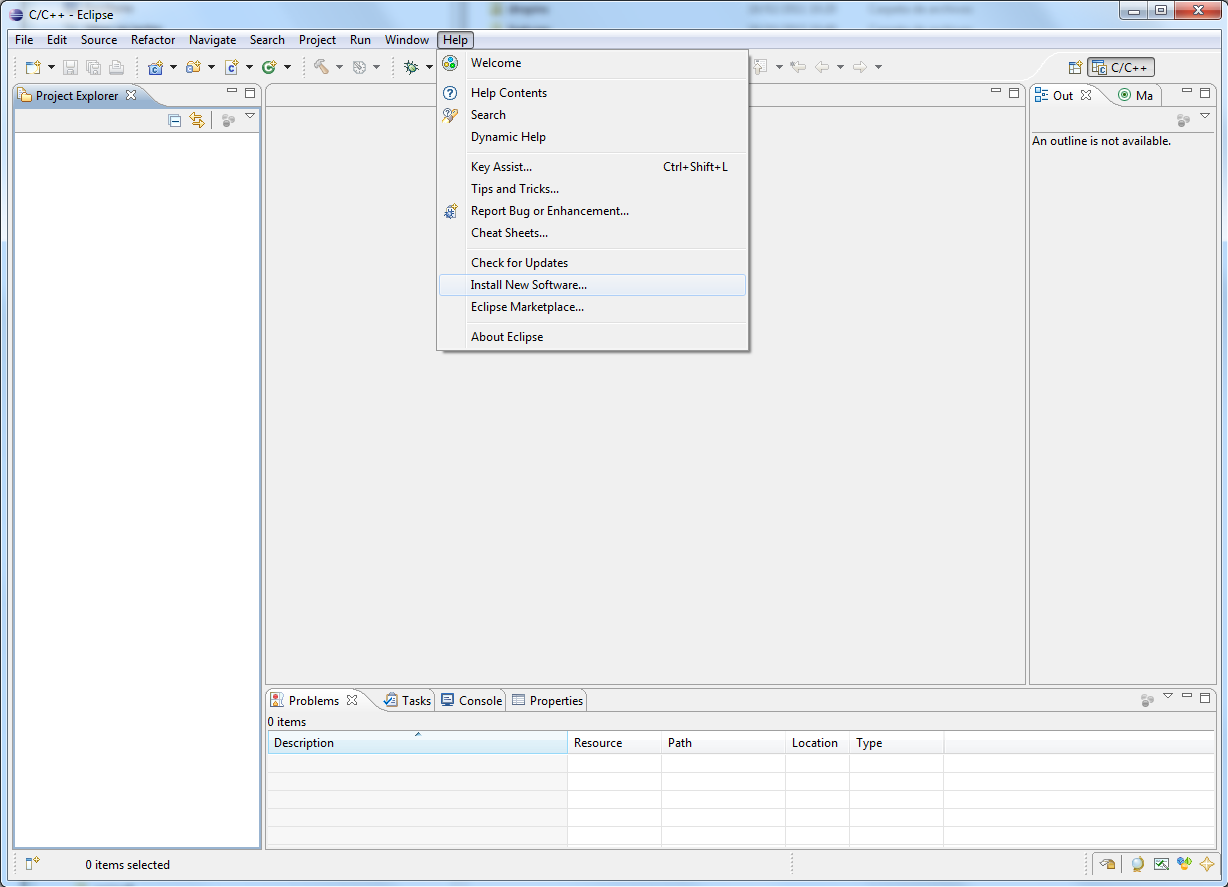
\includegraphics[height=9cm]{./Figuras/C2/c2_instalar_windows1.png}
\caption{Instalación del plugin NDS en eclipse (parte 1).}
\label{fig_c2_win1}
\end{figure}

A continuación en la ventana \textit{Available Software} se pulsa el botón \textit{Add}, y se introduce la siguiente información:
\begin{itemize}
	\item Name: \textit{NDS Manager builder}
	\item Location: \textit{http://dev.snipah.com/nds/updater}
\end{itemize}

Esta operación se refleja en la Figura \ref{fig_c2_win2}.

\begin{figure}[t]
\centering
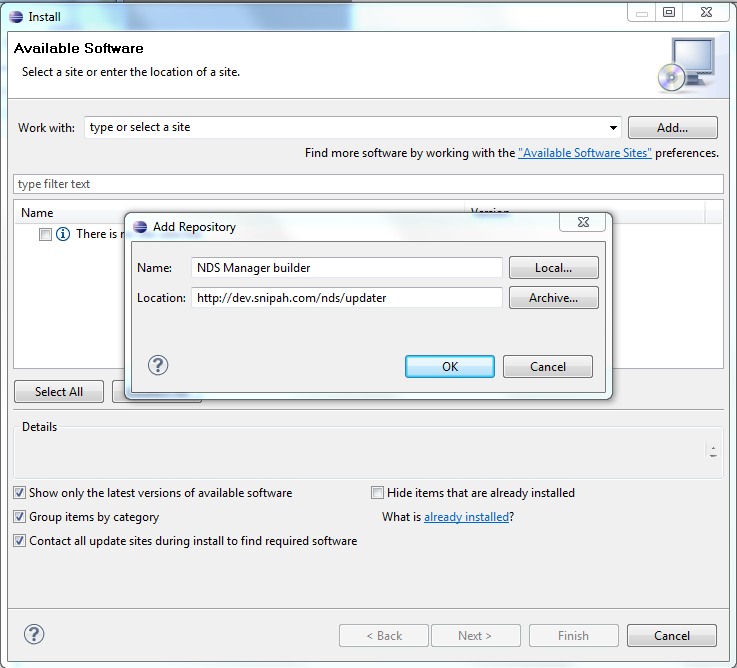
\includegraphics[height=8cm]{./Figuras/C2/c2_instalar_windows2.png}
\caption{Instalación del plugin NDS en eclipse (parte 2).}
\label{fig_c2_win2}
\end{figure}

Para que el proceso se realice de forma adecuada hay que tener la precaución de desactivar la opción \textit{Group items by category}. De esta forma aparecerá el software buscado, debiendo activarse las casillas correspondientes a \textit{devkitARM}, tal y como muestra la Figura \ref{fig_c2_win4}.

\begin{figure}[t]
\centering
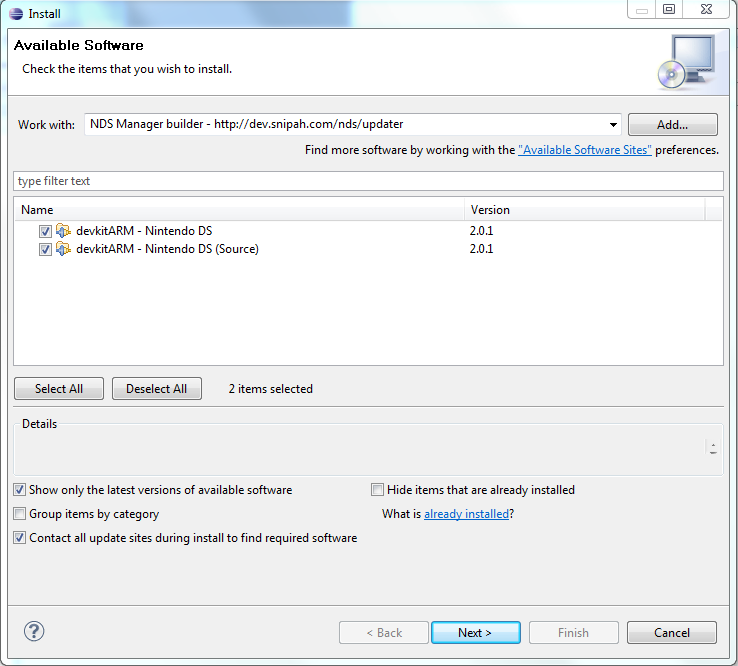
\includegraphics[height=8cm]{./Figuras/C2/c2_instalar_windows4.png}
\caption{Instalación del plugin NDS en eclipse (parte 3).}
\label{fig_c2_win4}
\end{figure}

Después de pulsar en sucesivos botones \textit{Next} y aceptar la licencia, comienza la instalación  del software. Durante dicho proceso puede aparecer la Figura \ref{fig_c2_win6}.

\begin{figure}[t]
\centering
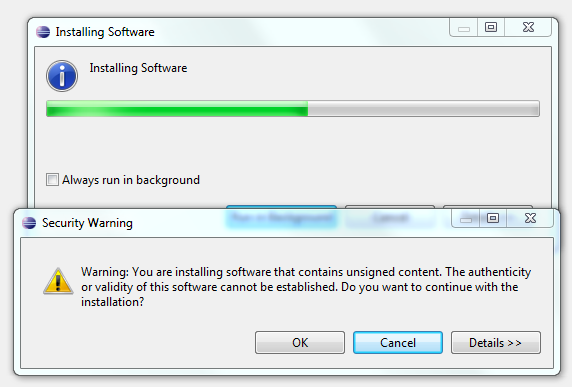
\includegraphics[height=7cm]{./Figuras/C2/c2_instalar_windows6.png}
\caption{Instalación del plugin NDS en eclipse (parte 4).}
\label{fig_c2_win6}
\end{figure}

Simplemente se pulsa en \textit{OK} para continuar el proceso de instalación. Una vez finalizada la instalación se debe reiniciar \textit{eclipse}.

Como comprobación de que todo ha ido correctamente, a la hora de crear el proyecto se debe observar que aparece algo parecido a lo mostrado en la Figura \ref{fig_c2_win7}.

\begin{figure}[h]
\centering
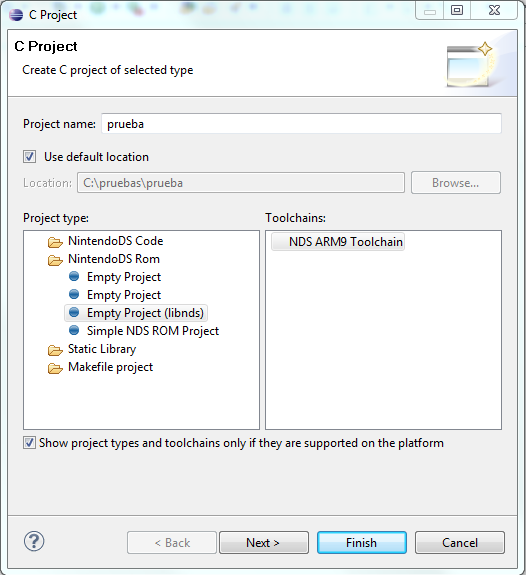
\includegraphics[height=8cm]{./Figuras/C2/c2_instalar_windows7.png}
\caption{Instalación del plugin NDS en eclipse (parte 5).}
\label{fig_c2_win7}
\end{figure}


Se elige \textit{Empty Project (libnds)}, y si después de pulsar en \textit{Next} aparece lo mostrado en la Figura \ref{fig_c2_win8}, entonces todo está correcto.

\newpage

\begin{figure}[h]
\centering
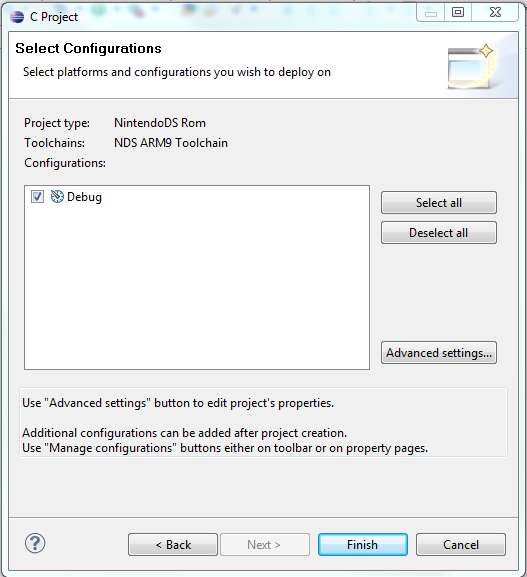
\includegraphics[height=8cm]{./Figuras/C2/c2_instalar_windows8.png}
\caption{Instalación del plugin NDS en eclipse (parte 6).}
\label{fig_c2_win8}
\end{figure}


% --------------------------------------------------------------------------
% --------------------------------------------------------------------------
% --------------------------------------------------------------------------
% --------------------------------------------------------------------------
\section{Nuestro primer programa para NDS en Windows}
En esta sección se van a ver los pasos para realizar nuestro primer programa para la NDS en el sistema operativo \textit{Windows}. 

% --------------------------------------------------------------------------
% --------------------------------------------------------------------------

\subsection{Desarrollar código para la NDS sin emplear Eclipse}
\label{sec:programa}
En este apartado se va a crear el primer programa en la NDS sin emplear \textit{Eclipse} como herramienta de desarrollo.

% --------------------------------------------------------------------------
\subsubsection{Creación de la estructura de ficheros}
Se puede emplear como punto de partida el ejemplo  \textit{hello\_world} que aparece en el directorio \textit{nds} del directorio \textit{examples} de  \textit{DevkitPro}. En  el laboratorio de prácticas, \textit{DevkitPro} se encuentra en el directorio \textit{C:$\backslash$}. En el directorio donde se vayan a almacenar los  programas a desarro\-llar se crea un nuevo directorio que identifique el programa a desarrollar (p.ej. \textit{ejemplo}). Dentro de ese directorio se crea el directorio \textit{source}, que contendrá los ficheros necesarios para el código a desarrollar (p.ej. \textit{main.c}). En el directorio \textit{ejemplo} se copia el fichero \textit{Makefile} del  ejemplo  \textit{hello\_world} de \textit{DevkitPro}. De esta forma la estructura de ficheros que se tiene es la siguiente:

{\scriptsize
 \begin{verbatim}
  c:\mis_ejemplos
    - directorio ejemplo
      - fichero Makefile
      - directorio source
        - fichero main.c
\end{verbatim}
}

% --------------------------------------------------------------------------
\subsubsection{Edición del fichero ejemplo}
Para familiarizarse con el entorno de desarrollo de aplicaciones para Nintendo DS, se va a utilizar como ejemplo una aplicación en la que aparezca un saludo con el nombre del desarrollador del programa. Para escribir este código se puede emplear cualquier editor de texto. Según esto, el código del programa a desarrollar (\textit{main.c}) es el siguiente:

\begin{lstlisting}
#include<nds.h>
#include<stdio.h>
int main(void) {
    consoleDemoInit();
    iprintf("Hola mundo");  // Imprimir el mensaje 
    while(1) {} // Bucle que no hace nada.     
}
\end{lstlisting}

En dicho código cabe destacar lo siguiente:
\begin{itemize}
\item \textit{consoleDemoInit}: inicializa una consola de texto predeterminada, sin permitir elegir la pantalla donde se imprimie el texto. En este caso, será la pantalla inferior de la videoconsola. Se verán más detalles de cómo seleccionar la pantalla en la que se visualiza información en prácticas posteriores. 
%
\item  \textit{iprintf("Hola mundo")}: esta función imprime texto con formato, soportando solo números enteros.
\end{itemize}

% --------------------------------------------------------------------------
\subsubsection{Compilación del fichero ejemplo}
El siguiente paso es compilar el programa, para ello se abre el \textit{símbolo del sistema}. Una vez se está en el directorio \textit{ejemplo} creado, se ejecuta el comando \textit{make}:

{\scriptsize
\begin{verbatim}
 C:\mis_ejemplos\ejemplo>dir
 29/07/2013  15:10    <DIR>          .
 29/07/2013  15:10    <DIR>          ..
 02/04/2012  22:02             4.903 Makefile
 29/07/2013  15:10    <DIR>          source
                1 archivos          4.903 bytes
                3 dirs  51.779.096.576 bytes libres
 \end{verbatim}
}

{\scriptsize
\begin{verbatim}
 C:\mis_ejemplos\ejemplo>make
 main.c
 arm-none-eabi-gcc -MMD -MP -MF /d/mis_ejemplos/ejemplo/build/main.d -g -Wall 
 -O2 -march=armv5te -mtune=arm946e-s -fomit-frame-pointer -ffast-ma
 th -mthumb -mthumb-interwork -I/d/mis_ejemplos/ejemplo/include
 -I/d/mis_ejemplos/ejemplo/build -I/c/devkitPro/libnds/include 
 -I/d/mis_ejemplos/ejemplo/build -DARM9 -c /d/mis_ejemplos/ejemplo/source/main.c 
 -o main.o
 linking ejemplo.elf
 Nintendo DS rom tool 1.50.1 - Jun 19 2012
 by Rafael Vuijk, Dave Murphy, Alexei Karpenko
 built ... ejemplo.nds
\end{verbatim}
}

Si no se han producido errores de compilación aparecerán los ficheros  \textit{ejemplo.elf} y \textit{ejemplo.nds}.

{\scriptsize
 \begin{verbatim}
 C:\mis_ejemplos\ejemplo>dir
 29/07/2013  15:15    <DIR>          .
 29/07/2013  15:15    <DIR>          ..
 29/07/2013  15:15    <DIR>          build
 29/07/2013  15:15           234.949 ejemplo.elf
 29/07/2013  15:15           134.208 ejemplo.nds
 02/04/2012  22:02             4.903 Makefile
 29/07/2013  15:10    <DIR>          source
                3 archivos        374.060 bytes
                4 dirs  51.778.568.192 bytes libres
 \end{verbatim}
}

El primero (\textit{ejemplo.elf}) es el que contiene la información de depuración, por tanto, el depurador tendrá que trabajar necesariamente con él. Sin embargo,  la consola (o el emulador) solo será capaz de ejecutar la imagen del cartucho \textit{ejemplo.nds}. También se ha creado el directorio \textit{build}, que por ahora no tiene interés para lo que se  se está desarrollando. Para borrar todos los ficheros y directorios creados durante la compilación se puede ejecutar \textit{make clean}.

Si se produjese un error relacionado con que no encuentra el compilador se puede realizar lo siguiente:
\begin{itemize}
\item Hacer una copia de los siguientes ficheros que se encuentran en \textit{C:$\backslash$devkitPro$\backslash$devkitARM$\backslash$bin}:	
	\begin{itemize}
 		\item arm-none-eabi-as
 		\item arm-none-eabi-g++
	 	\item arm-none-eabi-gcc	
 		\item arm-none-eabi-gdb
	   \item arm-none-eabi-objcopy
	\end{itemize}
\item Renombrar las copias con los siguientes nombres:	
	\begin{itemize}
		\item arm-eabi-as
	 	\item arm-eabi-g++
	 	\item arm-eabi-gcc	
 		\item arm-eabi-gdb
	   \item arm-eabi-objcopy
	\end{itemize}
\end{itemize}

% --------------------------------------------------------------------------
\subsubsection{Ejecución del fichero ejemplo en el emulador}
Si no se ha producido ningún problema en la compilación, la salida del programa se puede ver en el emulador. Una vez abierto \textit{WinDS Pro}, si se escoge el emulador \textit{No\$gba}, se pulsa en \textit{File->Cartridge Menu (File Name)} y se busca el fichero \textit{.nds} que nos interesa. En nuestro caso, y una vez elegido \textit{ejemplo.nds} aparece la ventana en el emulador mostrada en la Figura \ref{fig_c2_eclipse11b}.

\begin{figure}[h]
\centering
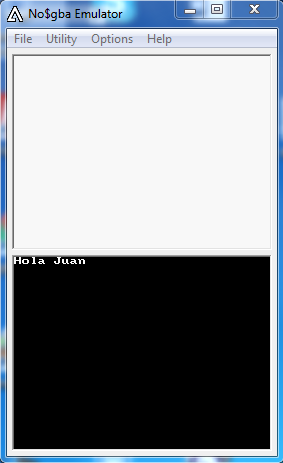
\includegraphics[height=8cm]{./Figuras/C2/c2_eclipse11b.png}
\caption{Ejecución del programa ejemplo en el emulador \textit{No\$gba}.}
\label{fig_c2_eclipse11b}
\end{figure}

Si se escoge el emulador \textit{DeSmuME}, se pulsa en \textit{File->Open ROM} y se busca el fichero \textit{.nds} que nos interesa.

% --------------------------------------------------------------------------
% --------------------------------------------------------------------------
\subsection{Desarrollar código para la NDS empleando Eclipse}
\label{sin_eclipse}
En este apartado se va a crear el primer programa en la NDS empleando \textit{Eclipse} como herramienta de desarrollo.

% --------------------------------------------------------------------------
\subsubsection{Creación de un proyecto para NDS}
En  el laboratorio de prácticas, \textit{Eclipse} se encuentra en el directorio \textit{C:$\backslash$}. Al iniciar \textit{Eclipse} se pide el directorio donde se almacenará el proyecto a crear, tal como muestra la Figura \ref{fig_c2_eclipse1}.

\begin{figure}[t]
\centering
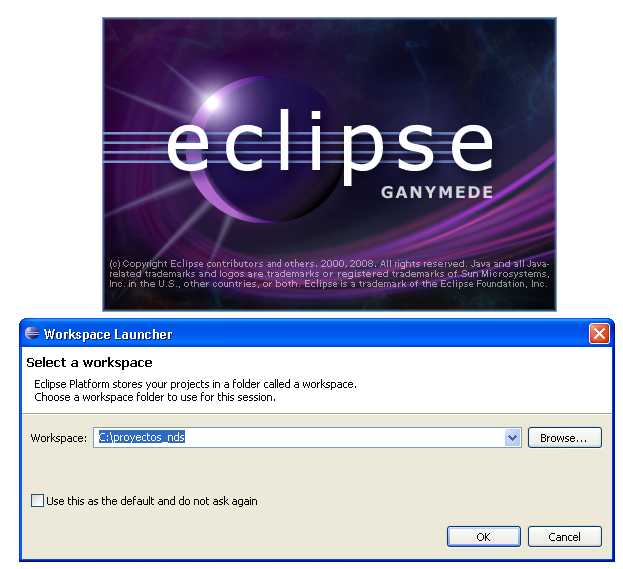
\includegraphics[height=9cm]{./Figuras/C2/c2_eclipse1.png}
\caption{Creación de un proyecto para NDS usando Eclipse (parte 1).}
\label{fig_c2_eclipse1}
\end{figure}


Para crear un nuevo proyecto se debe pulsar en la ventana principal de \textit{Eclipse} en \textit{File->New->C project} (ver Figura \ref{fig_c2_eclipse2}). 

\begin{figure}[t]
\centering
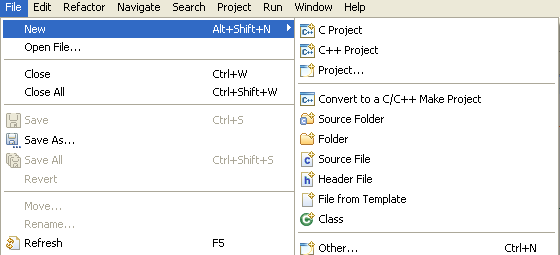
\includegraphics[height=6cm]{./Figuras/C2/c2_eclipse2.png}
\caption{Creación de un proyecto para NDS usando Eclipse (parte 2).}
\label{fig_c2_eclipse2}
\end{figure}

Aparece la ventana (\textit{C Project}) mostrada en la Figura \ref{fig_c2_eclipse3}.

\begin{figure}[t]
\centering
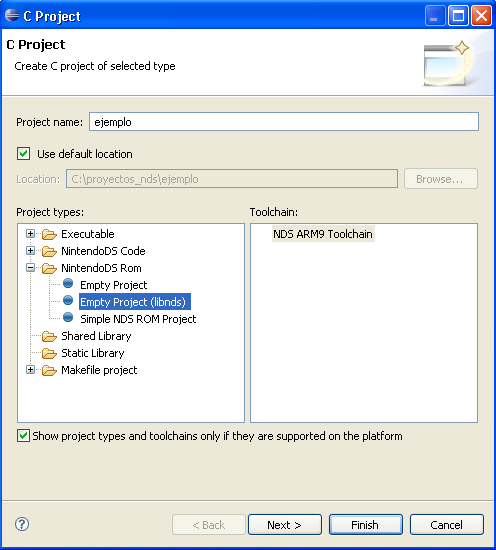
\includegraphics[height=8cm]{./Figuras/C2/c2_eclipse3.png}
\caption{Creación de un proyecto para NDS usando Eclipse (parte 3).}
\label{fig_c2_eclipse3}
 \end{figure}

\noindent en la que se debe configurar lo siguiente:
\begin{itemize}
\item El nombre del proyecto (p.ej. \textit{ejemplo}).
\item En \textit{Project types} se selecciona \textit{Nintendo DS Rom-> Empty Project (libnds)}.
\item Se pulsa en \textit{Next}.
\end{itemize}

Aparece una ventana de \textit{Select Configurations} en la que se pulsa en \textit{Finish}. 

Una vez creado el proyecto, si lo que aparece es la siguiente ventana se debe elegir el icono de \textit{workbench}, tal y como se muestra en la Figura \ref{fig_c2_eclipsew}.

\begin{figure}[t]
\centering
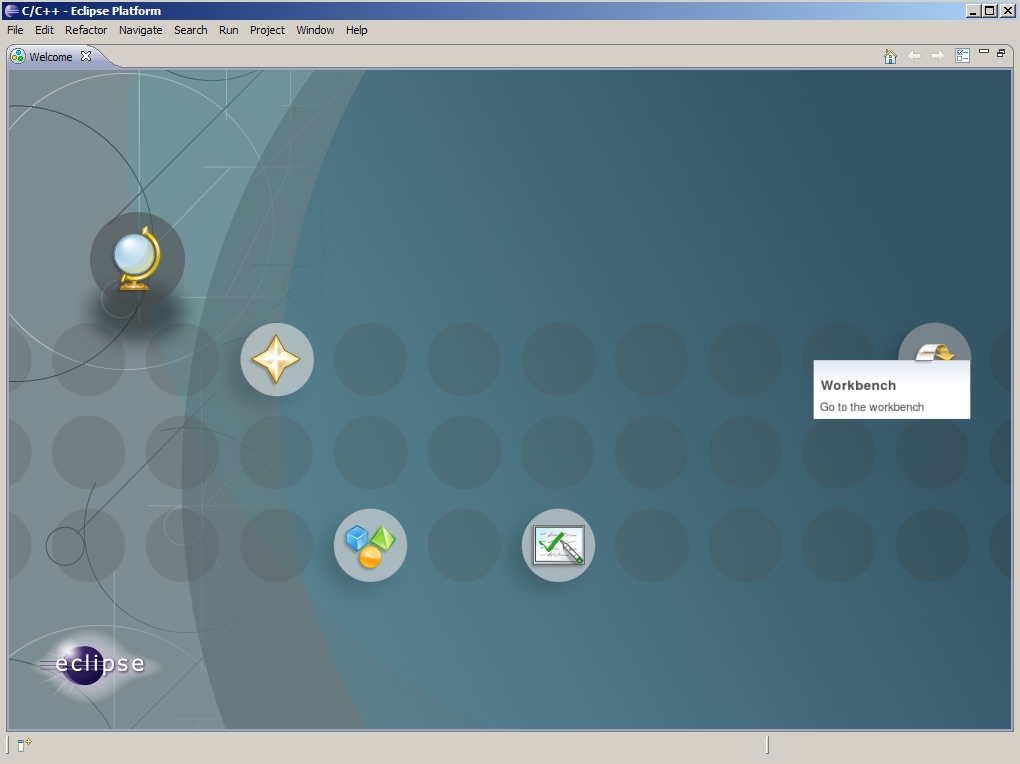
\includegraphics[height=8cm]{./Figuras/C2/c2_eclipse-workbench.png}
\caption{Creación de un proyecto para NDS usando Eclipse  (parte 4).}
\label{fig_c2_eclipsew}
\end{figure}

De esta forma, el  proyecto creado aparecerá en la ventana de \textit{workbench} de \textit{Eclipse} (ver Figura \ref{fig_c2_eclipse4}).

\begin{figure}[t]
\centering
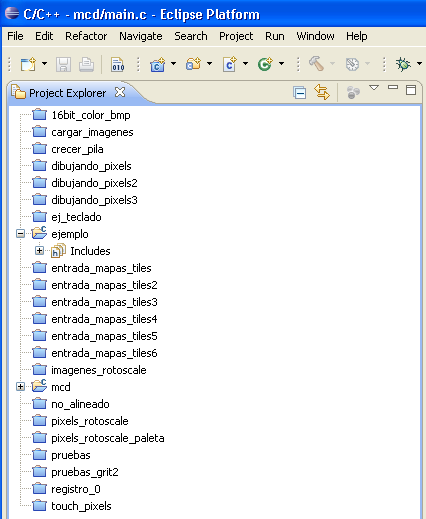
\includegraphics[height=8cm]{./Figuras/C2/c2_eclipse4.png}
\caption{Creación de un proyecto para NDS usando Eclipse (parte 5).}
\label{fig_c2_eclipse4}
\end{figure}

Esta ventana podría aparecer directamente sin necesidad de elegir el icono de \textit{workbench} de \textit{Eclipse}.

% --------------------------------------------------------------------------
\subsubsection{Configuración del proyecto}
Para iniciar la configuración del proyecto, se debe pulsar en la ventana principal de \textit{Eclipse} en \textit{Project Properties}, teniendo la precaución de tener activado el proyecto que se desea. Una vez realizada esta operación aparece la ventana (\textit{Properties for ejemplo}) (ver Figura \ref{fig_c2_eclipse5}).

\begin{figure}[t]
\centering
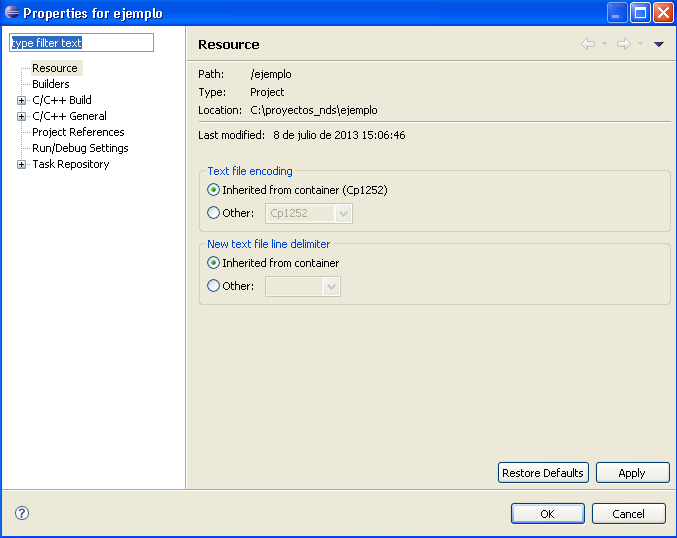
\includegraphics[height=8cm]{./Figuras/C2/c2_eclipse5.png}
\caption{Creación de un proyecto para NDS usando Eclipse (parte 6).}
\label{fig_c2_eclipse5}
\end{figure}

En dicha ventana se debe desplegar la pestaña \textit{C/C++ Build}. Se resalta dicha opción. En el cuadro \textit{Builder} de la pestaña \textit{Builder Settings} se cambia la opción \textit{Builder Type} a \textit{Internal Builder} (ver Figura \ref{fig_c2_eclipse6}).

\begin{figure}[t]
	\centering
	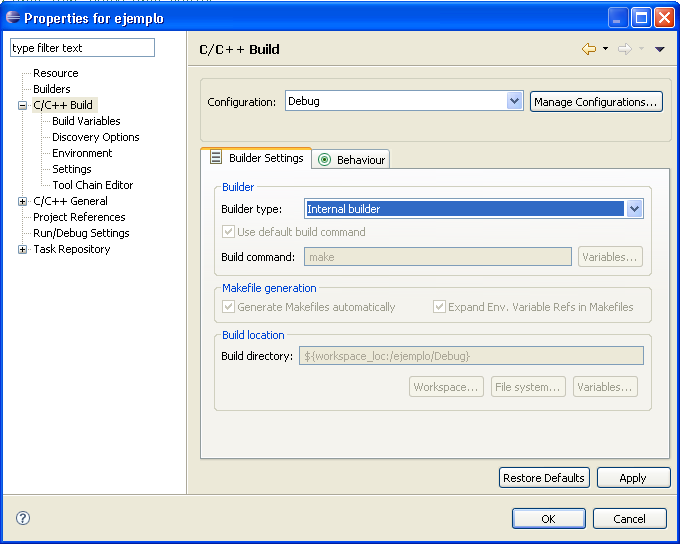
\includegraphics[height=8cm]{./Figuras/C2/c2_eclipse6.png}
	\caption{Creación de un proyecto para NDS usando Eclipse (parte 7).}
	\label{fig_c2_eclipse6}
\end{figure}

En la pestaña \textit{C/C++ Build} se resalta \textit{Settings}, apareciendo la ventana que se muestra en la Figura \ref{fig_c2_eclipse7}.

\begin{figure}[t]
	\centering
	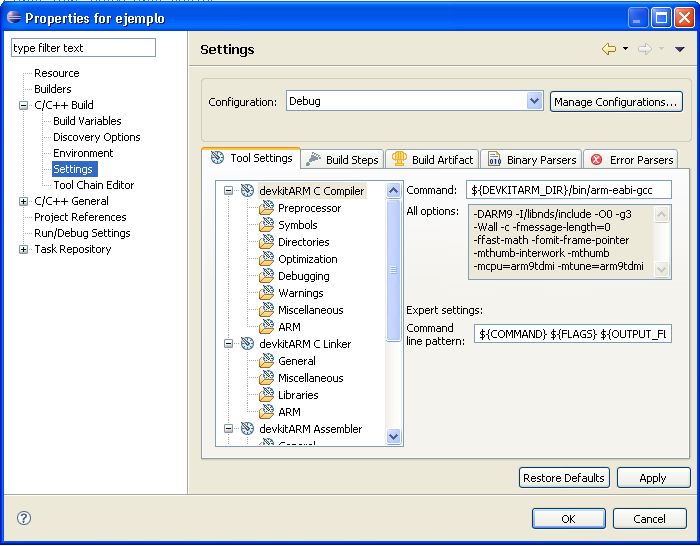
\includegraphics[height=8cm]{./Figuras/C2/c2_eclipse7.png}
	\caption{Creación de un proyecto para NDS usando Eclipse  (parte 8).}
	\label{fig_c2_eclipse7}
\end{figure}

Se escoge \textit{devkitARM C Linker->ARM} y se desactiva la opción \textit{No FPU}. En NDSTool se debe poner el comando \textit{\$\{DEVKITPRO\_DIR\}/tools/bin/ndstool}. Finalmente se pulsa en \textit{OK} (ver Figura \ref{fig_c2_eclipse8}).

\begin{figure}[t]
	\centering
	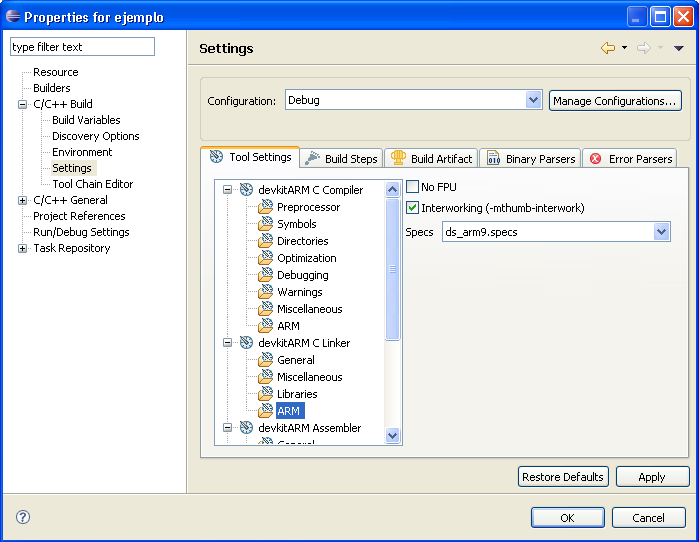
\includegraphics[height=8cm]{./Figuras/C2/c2_eclipse8.png}
	\caption{Creación de un proyecto para NDS usando Eclipse  (parte 9).}
	\label{fig_c2_eclipse8}
\end{figure}

% --------------------------------------------------------------------------
\subsubsection{Edición del fichero ejemplo}
Para familiarizarse con el entorno de desarrollo de \textit{Eclipse} para NDS, se utiliza el mismo ejemplo que el del apartado anterior. En primer lugar, se debe crear un fichero fuente en \textit{lenguaje C} dentro del proyecto actual. Para ello se pulsa en \textit{File->New->Source File} (ver Figura \ref{fig_c2_eclipse9}).

\begin{figure}[t]
	\centering
	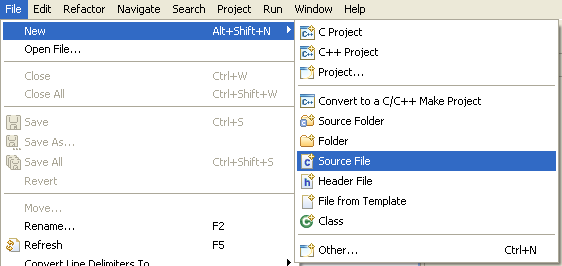
\includegraphics[height=7cm]{./Figuras/C2/c2_eclipse9.png}
	\caption{Creación de un proyecto para NDS usando Eclipse  (parte 10).}
	\label{fig_c2_eclipse9}
\end{figure}

Aparece una nueva ventana (\textit{New Source File}) (ver Figura \ref{fig_c2_eclipse10}).

\begin{figure}[t]
	\centering
	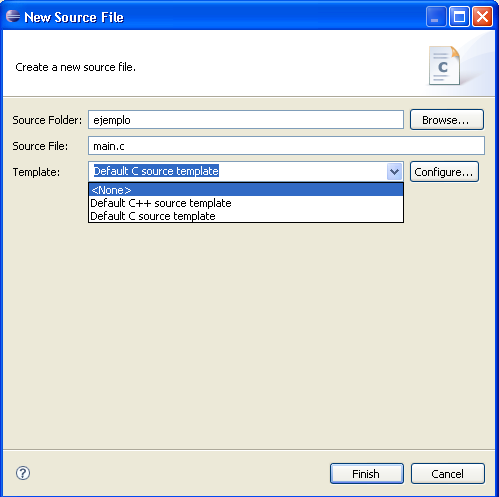
\includegraphics[height=7cm]{./Figuras/C2/c2_eclipse10.png}
	\caption{Creación de un proyecto para NDS usando Eclipse  (parte 11).}
	\label{fig_c2_eclipse10}
\end{figure}


\noindent en la que se debe realizar lo siguiente:
\begin{itemize}
 	\item En \textit{Source File} se introduce \textit{main.c}.
 	\item En \textit{Template} se selecciona \textit{None}.
 	\item Se pulsa en \textit{Finish}.
\end{itemize}

A continuación en la ventana que hace referencia a \textit{main.c} se introduce el mismo código que el del apartado \ref{sec:programa}.

% --------------------------------------------------------------------------
\subsubsection{Compilación del fichero ejemplo}
El siguiente paso es compilar el programa, para ello se elige \textit{Project->Build Project}. Si no se han producido errores de compilación aparecerán los ficheros  \textit{ejemplo.elf} y \textit{ejemplo.nds} en el directorio \textit{Debug}, tal y como se puede comprobar en la Figura \ref{fig_c2_ficheros_eclipse}.

\begin{figure}[t]
	\centering
	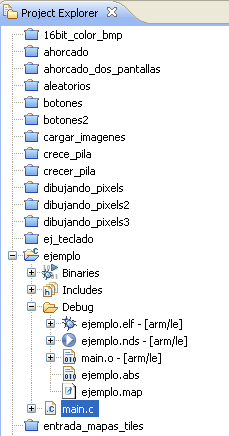
\includegraphics[height=7cm]{./Figuras/C2/c2_ficheros_eclipse.png}
	\caption{Creación de un proyecto para NDS usando Eclipse  (parte 12).}
	\label{fig_c2_ficheros_eclipse}
\end{figure}

Si se produjese un error relacionado con que no encuentra el compilador se puede realizar lo siguiente:
\begin{itemize}
\item Hacer una copia de los siguientes ficheros que se encuentran en \textit{C:$\backslash$ devkitPro $\backslash$ devkitARM $\backslash$ bin}:	
	\begin{itemize}
	 	\item arm-none-eabi-as
	 	\item arm-none-eabi-g++
	 	\item arm-none-eabi-gcc	
	 	\item arm-none-eabi-gdb
	   \item arm-none-eabi-objcopy
	\end{itemize}
\item Renombrar las copias con los siguientes nombres:	
	\begin{itemize}
	 	\item arm-eabi-as
	 	\item arm-eabi-g++
	 	\item arm-eabi-gcc	
	 	\item arm-eabi-gdb
	   \item arm-eabi-objcopy
	 \end{itemize}
\end{itemize}


% --------------------------------------------------------------------------
\subsubsection{Ejecución del fichero ejemplo en el emulador}
Una vez abierto \textit{WinDS Pro}, si se escoge el emulador \textit{No\$gba}, se pulsa en \textit{File->Cartridge Menu (File Name)} y se busca el fichero \textit{.nds} que nos interesa. En nuestro caso, y una vez elegido \textit{ejemplo.nds} aparece la ventana en el emulador mostrada en la Figura \ref{fig_c2_eclipse11b}.

Si se escoge el emulador \textit{DeSmuME}, se pulsa en \textit{File->Open ROM} y se busca el fichero \textit{.nds} que nos interesa.

% --------------------------------------------------------------------------
% --------------------------------------------------------------------------
% --------------------------------------------------------------------------
% --------------------------------------------------------------------------
\section{Instalación del entorno de desarrollo en Linux}
Las operaciones a seguir para instalar el entorno de desarrollo en Linux son las siguientes:

\begin{enumerate}
\item Instalación de \textit{devkitpro}. Se accede a la página web:
 	\begin{verbatim}
 	http://devkitpro.org/
 	\end{verbatim}
Se pulsa en \textit{For instructions on installing the toolchains see our Getting Started pages} y posteriormente elegir \textit{Manual instructions for installing devkitARM} y seguir los pasos que aparecen en dicha página web.
%	
\item Instalación de \textit{WinDS Pro}. Se puede descargar la última versión de \textit{WinDS Pro} de la siguiente página web:
	\begin{verbatim}
	 https://windsprocentral.blogspot.com.es/2016/10/winds-pro.html
	\end{verbatim} 
%
\item Instalación de \textit{desmume}. Se pueden seguir los pasos que aparecen en la siguiente página web:
{\scriptsize
	\begin{verbatim}
		http://wiki.desmume.org/index.php?title=Installing_DeSmuME_from_source_on_Linux
	\end{verbatim}
}

Recomendable emplear la opción \textit{Install desmume from svn}.
%
\item Instalación de \textit{eclipse} \textit{Helios}. Se siguen los mismos pasos que los indicados para Windows.
%
\item Instalación del \textit{plugin NDS ManagedBuilder}. En este caso será necesario  instalar el plugin mediante el actualizador del propio Eclipse que se encuentra en \textit{Help->Install New Software}. Para ello se emplea la \textit{url} de actualizaciones del \textit{NDS Managed builder}
 \textit{(http://dev.snipah.com/nds/updater)}, que se deberá especificar en la ventana mostrada en la Figura \ref{fig_c2_managebuilder}.
\end{enumerate}

\begin{figure}[t]
	\centering
	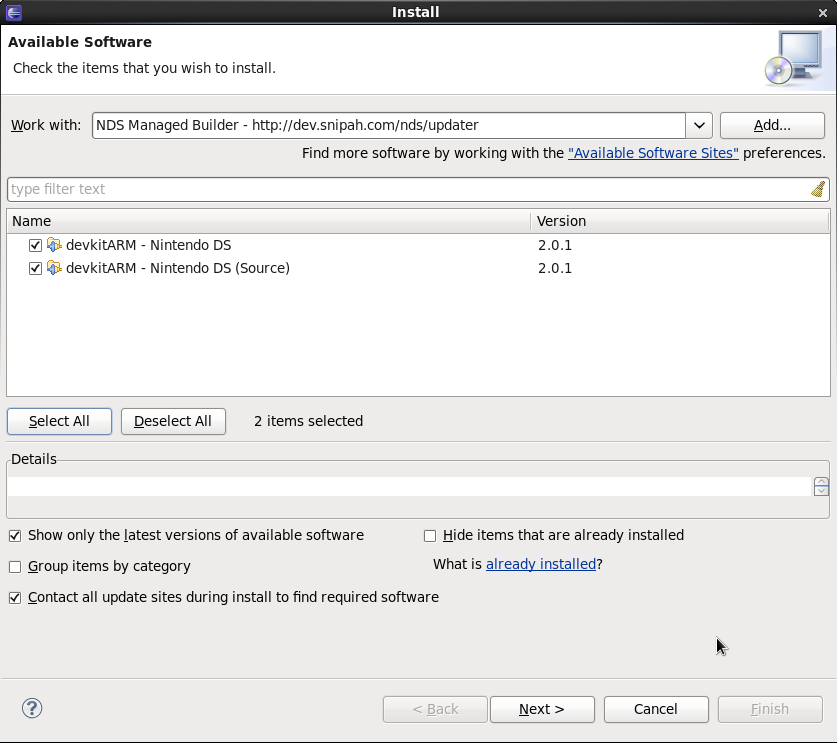
\includegraphics[height=8cm]{./Figuras/C2/c2_Pantallazo2.png}
	\caption{Instalación del \textit{plugin NDS ManagedBuilder}}
	\label{fig_c2_managebuilder}
\end{figure}


Hay que tener la precaución de desactivar la opción \textit{Group items by category}. Después de aceptar la licencia se instalará el plugin. Una vez finalizada la instalación se debe reiniciar Eclipse.

% --------------------------------------------------------------------------
% --------------------------------------------------------------------------
\section{Nuestro primer programa para NDS en Linux}
En esta sección se van a ver los pasos para realizar nuestro primer programa para la NDS en el sistema operativo \textit{Linux}. \textbf{En el laboratorio se debe entrar con la cuenta \textit{usuario}}. Antes de nada se debe comprobar que las siguientes variables de entorno se encuentran en el fichero \textit{.bash\_profile} del \textit{usuario}:
\begin{verbatim}
 export DEVKITPRO=/opt/devkitpro/
 export DEVKITARM=/opt/devkitpro/devkitARM/
\end{verbatim}

% --------------------------------------------------------------------------
% --------------------------------------------------------------------------
\subsection{Desarrollar código para la NDS sin emplear Eclipse}
En este apartado se va a crear el primer programa en la NDS sin emplear \textit{Eclipse} como herramienta de desarrollo.

% --------------------------------------------------------------------------
\subsubsection{Creación de la estructura de ficheros}
Se puede emplear como punto de partida el ejemplo  \textit{hello\_world} que aparece en el directorio \textit{nds} del directorio \textit{examples} de  \textit{DevkitPro}. En  el laboratorio de prácticas, \textit{DevkitPro} se encuentra en el directorio \textit{/opt/devkitpro}. En el directorio donde se vayan a almacenar los programas a desarro\-llar se crea un nuevo directorio que identifique el programa a desarrollar (p.ej. \textit{ejemplo}). Dentro de ese directorio se crea el directorio \textit{source}, que contendrá los ficheros necesarios para el código a desarrollar (p.ej. \textit{main.c}). En el directorio \textit{ejemplo} se copia el fichero \textit{Makefile} del  ejemplo  \textit{hello\_world} de \textit{DevkitPro}. De esta forma la estructura de ficheros que se tiene es la siguiente:
\begin{verbatim}
  /home/usuario/mis_ejemplos
    - directorio ejemplo
      - fichero Makefile
      - directorio source
        - fichero main.c
\end{verbatim}



% --------------------------------------------------------------------------
\subsubsection{Edición del fichero ejemplo}
Para familiarizarse con el entorno de desarrollo de aplicaciones para Nintendo DS, se va a utilizar como ejemplo una aplicación en la que aparezca un saludo con el nombre del desarrollador del programa. Para escribir este código se puede emplear cualquier editor de texto.

Según esto, el código del programa a desarrollar (\textit{main.c}) es el siguiente:
\begin{lstlisting}
#include<nds.h>
#include<stdio.h>
int main(void)
{
	consoleDemoInit();
    iprintf("Hola Juan");  // Imprimir el mensaje 
    while(1){} // Bucle que no hace nada.     
    return 0; // Finalizar el programa
}
\end{lstlisting}

% --------------------------------------------------------------------------
\subsubsection{Compilación del fichero ejemplo}
El siguiente paso es compilar el programa, para ello se abre el \textit{Terminal} \textit{(Sistema->Terminal)}. Una vez se está en el directorio \textit{ejemplo} creado, se ejecuta el comando \textit{make}:
\begin{verbatim}
 [usuario@labsop02 ejemplo]# make
 main.c
 arm-none-eabi-gcc -MMD -MP -MF /root/mis_ejemplos/ejemplo/build/main.d -g -Wall 
 -O2 -march=armv5te -mtune=arm946e-s -fomit-frame-pointer -ffast-math 
 -mthumb -mthumb-interwork -I/root/mis_ejemplos/ejemplo/include 
 -I/root/mis_ejemplos/ejemplo/build -I/opt/devkitpro//libnds/include 
 -I/root/mis_ejemplos/ejemplo/build -DARM9 -c 
 /root/mis_ejemplos/ejemplo/source/main.c -o main.o 
 linking ejemplo.elf
 Nintendo DS rom tool 1.50.1 - Jun 19 2012
 by Rafael Vuijk, Dave Murphy, Alexei Karpenko
 built ... ejemplo.nds
\end{verbatim}

Si no se han producido errores de compilación aparecerán los ficheros \textit{ejemplo.elf} y \textit{ejemplo.nds}.
\begin{verbatim}
 [usuario@labsop02 ejemplo]# ls -l
 total 332
 drwxr-xr-x 2 root root   4096 sep  5 18:01 build
 -rwxr-xr-x 1 root root 234909 sep  5 18:01 ejemplo.elf
 -rw-r--r-- 1 root root 134208 sep  5 18:01 ejemplo.nds
 -rwxr-xr-x 1 root root   4903 abr  2  2012 Makefile
 drwxr-xr-x 2 root root   4096 sep  5 18:00 source
                \end{verbatim}
Para borrar todos los ficheros y directorios creados durante la compilación se puede ejecutar \textit{make clean}.

Si se produjese un error relacionado con que no encuentra el compilador se puede realizar lo siguiente:
\begin{itemize}
\item Hacer una copia de los siguientes ficheros que se encuentran en \textit{/opt/devkitpro/devkitARM/bin}:	
	\begin{itemize}
 	\item arm-none-eabi-as
 	\item arm-none-eabi-g++
 	\item arm-none-eabi-gcc	
 	\item arm-none-eabi-gdb
    \item arm-none-eabi-objcopy
	\end{itemize}
\item Renombrar las copias con los siguientes nombres:	
	\begin{itemize}
 	\item arm-eabi-as
 	\item arm-eabi-g++
 	\item arm-eabi-gcc	
 	\item arm-eabi-gdb
    \item arm-eabi-objcopy
    \end{itemize}
\end{itemize}

% --------------------------------------------------------------------------
\subsubsection{Ejecución del fichero ejemplo en el emulador}
Si no se ha producido ningún problema en la compilación, la salida del programa se puede ver en el emulador. Una vez abierto \textit{WinDS Pro}, si se escoge el emulador \textit{No\$gba}, se pulsa en \textit{File->Cartridge Menu (File Name)} y se busca el fichero \textit{.nds} que nos interesa. Si se escoge el emulador \textit{DeSmuME}, se pulsa en \textit{File->Open ROM} y se busca el fichero \textit{.nds} que nos interesa.


% --------------------------------------------------------------------------
% --------------------------------------------------------------------------
\subsection{Desarrollar código para la NDS empleando Eclipse}
En este apartado se va a crear el primer programa en la NDS empleando \textit{Eclipse} como herramienta de desarrollo.

% --------------------------------------------------------------------------
\subsubsection{Creación de un proyecto para NDS}
En  el laboratorio de prácticas, \textit{Eclipse} se encuentra en el directorio \textit{/opt/eclipse-helios}.  Al iniciar \textit{Eclipse} se pide el directorio donde se almacenará el proyecto a crear (ver Figura \ref{fig_pig_p3_c1_eclipel1}).

\begin{figure}[t]
\centering
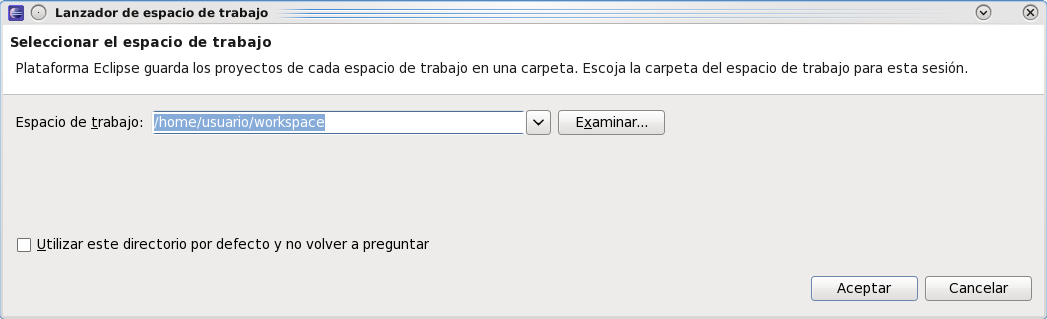
\includegraphics[height=4cm]{./Figuras/C2/c2_instan1.png}
\caption{Creación de un proyecto para NDS usando Eclipse en Linux (parte 1).}
\label{fig_pig_p3_c1_eclipel1}
 \end{figure}


Para crear un nuevo proyecto se debe pulsar en la ventana principal de \textit{Eclipse} en \textit{Archivo->Nuevo->Proyecto}.  Aparece la ventana (\textit{Proyecto nuevo}) mostrada en la Figura \ref{fig_pig_p3_c1_eclipel2}.

\begin{figure}[t]
	\centering
	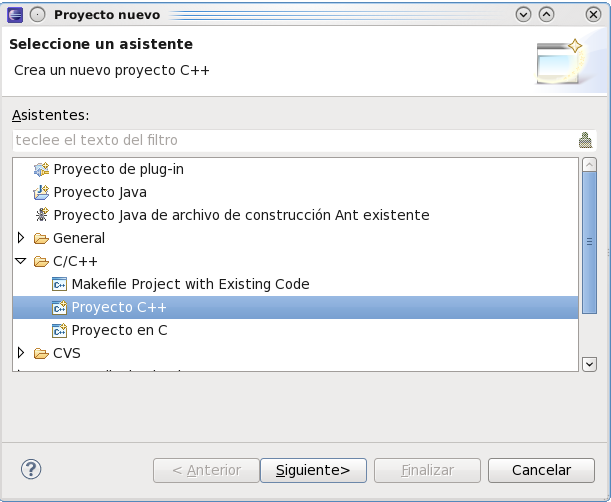
\includegraphics[height=8cm]{./Figuras/C2/c2_instan2.png}
	\caption{Creación de un proyecto para NDS usando Eclipse en Linux (parte 2).}
	\label{fig_pig_p3_c1_eclipel2}
\end{figure}

Se escoge \textit{C/C++->Proyecto en C} y se pulsa en \textit{Siguiente}, apareciendo la ventana \textit{Proyecto C} mostrada en la Figura \ref{fig_pig_p3_c1_eclipel3}.

\begin{figure}[t]
	\centering
	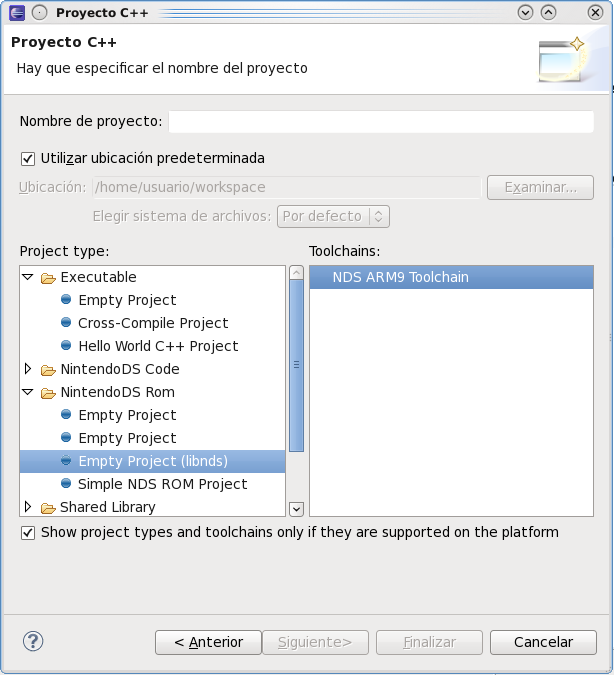
\includegraphics[height=8cm]{./Figuras/C2/c2_instan3.png}
	\caption{Creación de un proyecto para NDS usando Eclipse en Linux (parte 3).}
	\label{fig_pig_p3_c1_eclipel3}
\end{figure}

En dicha ventana se debe configurar lo siguiente:
 \begin{itemize}
 	\item El nombre de proyecto (p.ej. \textit{ejemplo}).
 	\item En \textit{Project type} se selecciona \textit{NintendoDS Rom-> Empty Project (libnds)}.
 	\item Se pulsa en \textit{Siguiente}.
 \end{itemize}

Aparece una ventana de \textit{Select Configurations} en la que se pulsa en \textit{Finalizar}. 

De esta forma, el  proyecto creado aparecerá en la ventana de \textit{workbench} de \textit{Eclipse}, lo que se muestra en la Figura \ref{fig_pig_p3_c1_eclipel4}.

\begin{figure}[t]
	\centering
	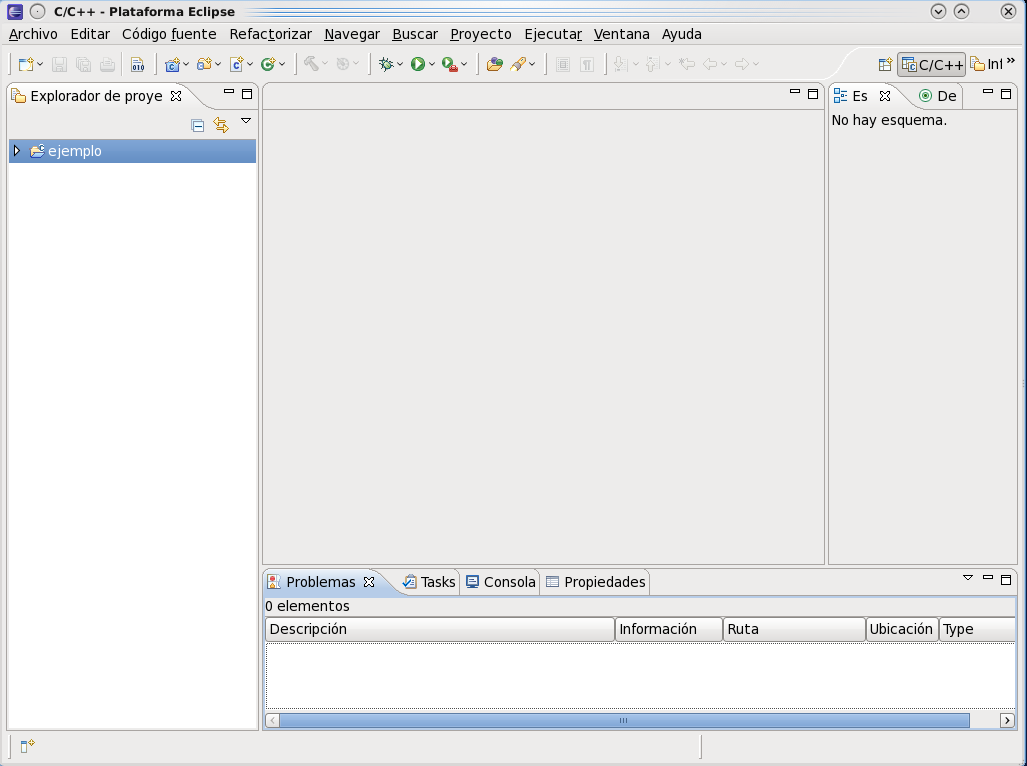
\includegraphics[height=8cm]{./Figuras/C2/c2_instan4.png}
	\caption{Creación de un proyecto para NDS usando Eclipse en Linux (parte 4).}
	\label{fig_pig_p3_c1_eclipel4}
\end{figure}

% --------------------------------------------------------------------------
\subsubsection{Configuración del proyecto}
Para iniciar la configuración del proyecto, se debe pulsar en la ventana principal de \textit{Eclipse} en \textit{Proyecto->Propiedades}, teniendo la precaución de tener activado el proyecto que se desea. Una vez realizada esta operación aparece la ventana (\textit{Propiedades de ejemplo}) (ver Figura \ref{fig_pig_p3_c1_eclipel5}).

\begin{figure}[t]
	\centering
	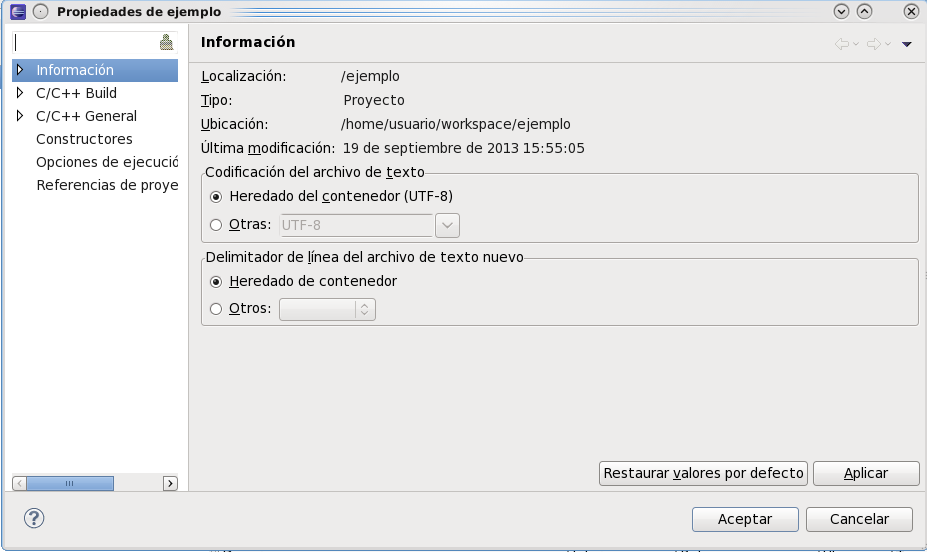
\includegraphics[height=8cm]{./Figuras/C2/c2_instan5.png}
	\caption{Creación de un proyecto para NDS usando Eclipse en Linux (parte 5).}
	\label{fig_pig_p3_c1_eclipel5}
\end{figure}

En dicha ventana se debe desplegar la pestaña \textit{C/C++ Build}. Se resalta dicha opción. En el cuadro \textit{Constructor} de la pestaña \textit{Builder Settings} se cambia la opción \textit{Builder Type} a \textit{Internal Builder} (ver Figura \ref{fig_pig_p3_c1_eclipel6}).


\begin{figure}[t]
	\centering
	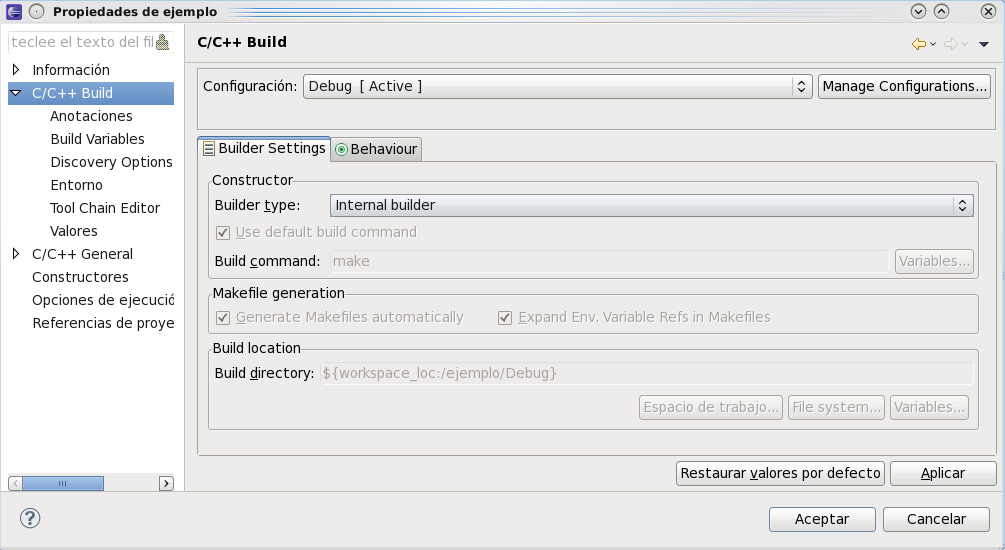
\includegraphics[height=8cm]{./Figuras/C2/c2_instan6.png}
	\caption{Creación de un proyecto para NDS usando Eclipse en Linux (parte 6).}
	\label{fig_pig_p3_c1_eclipel6}
\end{figure}

En la pestaña \textit{C/C++ Build} se resalta \textit{Valores}, apareciendo la ventana mostrada en la Figura \ref{fig_pig_p3_c1_eclipel7}.


\begin{figure}[t]
	\centering
	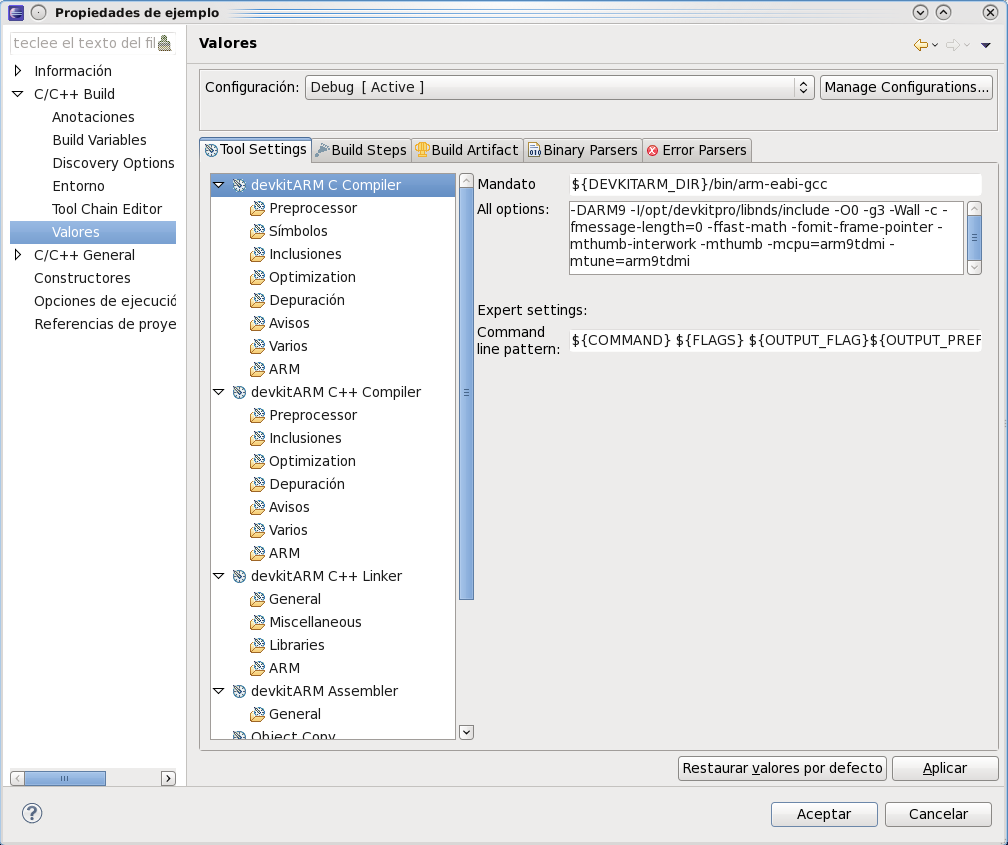
\includegraphics[height=7cm]{./Figuras/C2/c2_instan7.png}
	\caption{Creación de un proyecto para NDS usando Eclipse en Linux (parte 7).}
	\label{fig_pig_p3_c1_eclipel7}
\end{figure}

Se escoge \textit{devkitARM C Linker->ARM} y se desactiva la opción \textit{No FPU}. Finalmente se pulsa en \textit{Aceptar} (ver Figura \ref{fig_pig_p3_c1_eclipel8}).

\begin{figure}[t]
	\centering
	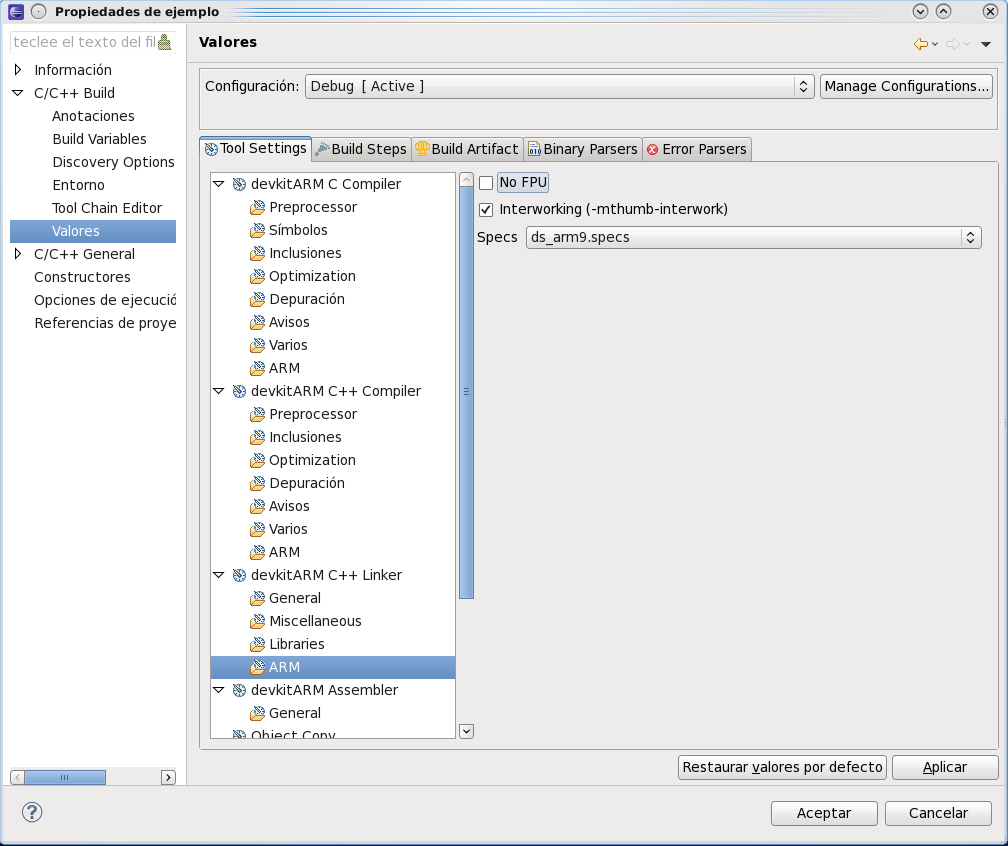
\includegraphics[height=7cm]{./Figuras/C2/c2_instan8.png}
	\caption{Creación de un proyecto para NDS usando Eclipse en Linux (parte 8).}
	\label{fig_pig_p3_c1_eclipel8}
\end{figure}


% --------------------------------------------------------------------------
\subsubsection{Edición del fichero ejemplo}
Para familiarizarse con el entorno de desarrollo de \textit{Eclipse} para NDS, se utiliza el mismo ejemplo que el del apartado anterior.  En primer lugar, se debe crear un fichero fuente en \textit{lenguaje C} dentro del proyecto actual. Para ello se pulsa en \textit{Archivo->Nuevo->Source File}. Aparece una nueva ventana (\textit{New Source File}) (ver Figura \ref{fig_pig_p3_c1_eclipel9}).

\begin{figure}[t]
	\centering
	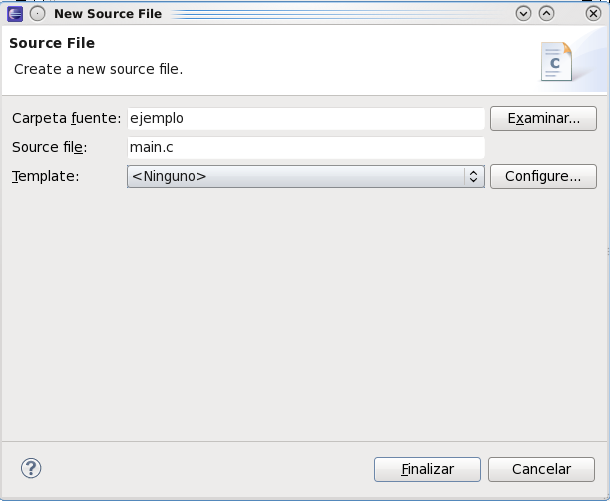
\includegraphics[height=7cm]{./Figuras/C2/c2_instan9.png}
	\caption{Creación de un proyecto para NDS usando Eclipse en Linux (parte 9).}
	\label{fig_pig_p3_c1_eclipel9}
\end{figure}


\noindent en la que se debe realizar lo siguiente:
\begin{itemize}
 	\item En \textit{Source File} se introduce \textit{main.c}.
 	\item En \textit{Template} se selecciona \textit{Ninguno}.
 	\item Se pulsa en \textit{Finalizar}.
\end{itemize}

A continuación en la ventana que hace referencia a \textit{main.c} se introduce el mismo código que el del apartado \ref{sec:programa}.

% --------------------------------------------------------------------------
\subsubsection{Compilación del fichero ejemplo}
El siguiente paso es compilar el programa, para ello se elige \textit{Proyecto->Construir proyecto}. Si no se han producido errores de compilación aparecerá el fichero \textit{ejemplo.nds} en el directorio \textit{Debug}. Si se produjese un error relacionado con que no encuentra el compilador se puede realizar lo siguiente:

\begin{itemize}
\item Hacer una copia de los siguientes ficheros que se encuentran en \textit{/opt/devkitpro/devkitARM/bin}:	
 \begin{itemize}
 	\item arm-none-eabi-as
 	\item arm-none-eabi-g++
 	\item arm-none-eabi-gcc	
 	\item arm-none-eabi-gdb
   \item arm-none-eabi-objcopy
 \end{itemize}
 	\item Renombrar las copias con los siguientes nombres:	
 \begin{itemize}
 	\item arm-eabi-as
 	\item arm-eabi-g++
 	\item arm-eabi-gcc	
 	\item arm-eabi-gdb
   \item arm-eabi-objcopy
 \end{itemize}
\end{itemize}

% --------------------------------------------------------------------------
\subsubsection{Ejecución del fichero ejemplo en el emulador}
Una vez abierto \textit{WinDS Pro}, si se escoge el emulador \textit{No\$gba}, se pulsa en \textit{File->Cartridge Menu (File Name)} y se busca el fichero \textit{.nds} que nos interesa. Si se escoge el emulador \textit{DeSmuME}, se pulsa en \textit{File->Open ROM} y se busca el fichero \textit{.nds} que nos interesa.

